\documentclass[12pt]{article}

\usepackage[margin=1in]{geometry}
\usepackage[pdftex]{hyperref}
\usepackage{amsmath,amsthm,amssymb,caption,graphicx,mathtools,hyperref,enumerate,enumitem}
\usepackage{centernot}
\usepackage{mdframed,cleveref}
\usepackage{bbm}
\usepackage[makeroom]{cancel}

\usepackage{svg}

\usepackage{pgf,tikz-cd,pgfplots}
\pgfplotsset{compat=1.15}
\usepackage{mathrsfs}
\usetikzlibrary{arrows}

\usepackage{multicol}

\usepackage{chngcntr}
\counterwithin{figure}{section}
\numberwithin{equation}{section}

\newtheoremstyle{break}% name
{}%         Space above, empty = `usual value'
{}%         Space below
{}% Body font
{}%         Indent amount (empty = no indent, \parindent = para indent)
{\bfseries}% Thm head font
{}%        Punctuation after thm head
{\newline}% Space after thm head: \newline = linebreak
{#1 #2 \normalfont #3}%         Thm head spec

\theoremstyle{definition}
\newtheorem*{remark}{Remark}

\theoremstyle{definition}
\newtheorem*{definition}{Definition}

\theoremstyle{definition}
\newtheorem*{theorem}{Theorem}

\theoremstyle{definition}
\newtheorem*{corollary}{Corollary}

\theoremstyle{break}
\newtheorem*{example}{Example}

\theoremstyle{definition}
\newtheorem*{lemma}{Lemma}

\theoremstyle{definition}
\newtheorem*{objective}{Objective}

\newmdenv[leftline=false,topline=false]{topright}
\let\proof\relax
\usepackage[utf8]{inputenc}
\usetikzlibrary{positioning}
\newcommand{\n}{\mathbb{N}}
\newcommand{\z}{\mathbb{Z}}
\newcommand{\q}{\mathbb{Q}}
\newcommand{\cx}{\mathbb{C}}
\newcommand{\real}{\mathbb{R}}
\newcommand{\E}{\mathbb{E}}
\newcommand{\V}{\mathbb{V}}
\newcommand{\bigo}{\mathcal{O}}
\newcommand{\divs}{\,\big|\,} %divides (a|b)
\newcommand{\bb}[1]{\mathbb{#1}}
\let\k\relax
\newcommand{\k}{\mathbf{k}}
\newcommand{\ita}[1]{\textit{#1}}
\newcommand\inv[1]{#1^{-1}}
\newcommand\setb[1]{\left\{#1\right\}}
\newcommand{\vbrack}[1]{\langle #1\rangle}
\newcommand{\determinant}[1]{\begin{vmatrix}#1\end{vmatrix}}
\newcommand{\abs}[1]{\left\vert #1 \right\vert}
\newcommand{\norm}[1]{\left\lVert#1\right\rVert}
\DeclareMathOperator{\Id}{Id}


\hypersetup{
	colorlinks,
	linkcolor=blue
}

\usepackage{tocloft} %table of contents package
\renewcommand{\cftsecleader}{\cftdotfill{\cftdotsep}}
\newcommand{\atoc}[1]{\addtocontents{toc}{#1\par}}

\setlength{\parindent}{0pt}

\title{Numerical Methods for Differential Equations}
\author{Ferran Arqué}
\date{2018}

\begin{document}

\maketitle

\tableofcontents

\atoc{\hyperref[sec:ode]{\color{black}\textbf{Ordinary Differential Equations}}}

\newpage
\section*{}\label{sec:ode}
\vspace*{\fill}
\hspace*{\fill}
\huge{ORDINARY DIFFERENTIAL EQUATIONS}
\hspace*{\fill}
\vspace*{\fill}
\normalsize
\newpage
\section{Ordinary Differential Equations. Basic concepts}

\subsection{Introduction and some notation}

Given $y' = f(x,y)$, where $\begin{cases} y(x) \in \real^n\\ f:\real\times\real^n \to \real^n\end{cases}$

\begin{definition}
  We denote by $y(x)$ the exact solution of the ODE system above.
\end{definition}

\begin{definition}
  $y_k$ is the approximation of $y(x_k)$ (after $k$ steps).
\end{definition}

\begin{objective}
  We want to approximate $y(x)$ within a given interval $[x_0, x_n]$. \\
  \footnotesize{
  \begin{multicols}{3}
    We know $\begin{cases}x_0\\x_1\\x_2\\\vdots\\x_n \end{cases}$\\
    \-\hspace{-2cm}We'd like to know $\begin{cases}y(x_0)\\y(x_1)\\y(x_2)\\\vdots \\y(x_n) \end{cases}$\\
    \-\hspace{-2cm}We find $\begin{cases} y_0\\y_1\\y_2\\\vdots \\y_n \end{cases}$ (given by a method)
  \end{multicols}
  }
\end{objective}
\normalsize
\begin{definition}
  $\norm{y(x_n) - y_n}$ is the \textbf{global error}.
\end{definition}

\begin{definition}
  We define the \textbf{local truncation error} as the error caused by one iteration, i.e. $$LTE = \norm{y(x_k) - y_k} \qquad \text{\big(assuming the \textit{localizing assumption}: $y_{k-1} = y(x_{k-1})$\big)}$$
\end{definition}

\begin{definition}
  A method is of \textbf{order} $p$ if the LTE is of the form $$\text{LTE} = Ch^{p+1} + \mathcal{O}(h^{p+2})$$
\end{definition}

\subsection{Euler's method}
\subsubsection{Formulation}
Consider the differential equation system
\begin{equation}\label{sys1.2}
  y'(x) = f(y(x)), \qquad y(x_0) = y_0 \qquad (\text{with } f:\real^n \to \real^n)
\end{equation}

We'll also assume, for later results, that $f$ satisfies a Lipschitz condition $$\norm{f(y) - f(z)} \leq L\norm{y-z}$$

Now, we want to find an approximation of (\ref{sys1.2}) on an interval $[x_0, x_N]$, so we'll create a set of $N+1$ evenly spaced points between $x_0$ and $x_N$, where $N$ is the number of steps and $h = \dfrac{x_N-x_0}{N}$ the stepsize.\\

To do that, we can use Euler's method
\[
  y_{n+1} = y_n + hf(y_n)
\]

\newpage

\subsubsection{Local truncation error}

We want to find $LTE = \norm{y(x_{n+1}) - y_{n+1}}$. Let's expand it

\begin{align*}
    y(x_{n+1}) - y_{n+1} &= y(x_n + h) - y_{n+1} = y(x_n) + hy'(x_n) + \mathcal{O}(h^2) - y_n - hf(y_n) \underset{\text{Loc.ass.}}{=} \\
    &= y(x_n)+ hy'(x_n) + \mathcal{O}(h^2) - y(x_n) - hf(y(x_n)) \\
    &= hy'(x_n) + \mathcal{O}(h^2) - hy'(x_n) = \mathcal{O}(h^2)
\end{align*}
  
So LTE = $\mathcal{O}(h^2)$, and the method has order $p=1$.

\subsubsection{Convergence}

For the method to be convergent, it has to verify $$\norm{y(x_N) - y_N} \underset{h\to0}{\longrightarrow} 0$$

Similar as what we did with the LTE, we'll find a bound for the error in one step, but this time without using the localizing assumption:

\begin{align*}
    \norm{y(x_{n+1}) - y_{n+1}} &= \norm{y(x_n + h) - y_n - hf(y_n)} \underset{\text{Taylor}}{=} ||y(x_n) + h\underbrace{y'(x_n)}_{f(y(x_n))} + \Tilde{c}h^2 - y_n - hf(y_n)|| \\
    &\leq \norm{y(x_n) - y_n} + h\underbrace{\norm{f(y(x_n)) - f(y_n)}}_{\substack{\text{\rotatebox{270}{$\leq$}} \\ L\norm{y(x_n) - y_n}}} + ch^2 \leq (1+hL)\norm{y(x_n) - y_n} + ch^2 \quad \forall n
\end{align*}

Thus
\begin{align*}
    &\norm{y(x_1) - y_1} \leq (1+hL)\norm{y(x_0) - y_0} + c_1h^2 \\
    &\norm{y(x_2) - y_2} \leq (1+hL)\norm{y(x_1) - y_1} + c_2h^2 \leq (1+hL)^2\norm{y(x_0) - y_0} + (1+hL)c_1h^2 + c_2h^2 \\
    &\norm{y(x_3) - y_3} \leq (1+hL)^3\norm{y(x_0) - y_0} + (1+hL)^2c_1h^2 + (1+hL)c_2h^2 + c_3h^2\\
    &\hspace{1.2cm}\vdots
\end{align*}
%\-\\
Let $C = \underset{i}{\text{max}}\,c_i$ \\

Then
\begin{align*}
    \norm{y(x_N) - y_N} \leq (1+hL)^N \norm{y(x_0) - y_0} + \underbrace{\Big(1 + (1+hL) + (1+hL)^2 + \ldots + (1+hL)^{N-1}\Big)}_{\substack{\text{\hspace{-0.94cm}geom$\to\,$\rotatebox{90}{$=$}}\\\frac{(1+hL)^N-1}{hL}}}Ch^2
\end{align*}

\[
  \implies \norm{y(x_n) - y_N} \leq (1+hL)^N\underbrace{\norm{y(x_0) - y_0}}_{\substack{\text{\hspace{-0.6cm}(\ref{sys1.2})\,\rotatebox{90}{=}}\\ 0}} + \frac{(1+hL)^N-1}{\cancel{h}L}\cdot Ch^{\cancel{2}} \leq Ah \to 0
\]

\begin{remark}
  In the last inequality we used $(1+hL)^N = e^{N\log(1+hL)} \underset{\substack{\log(1+x)\\\leq x + cx^2}}{\leq} e^{N(hL + ch^2L^2)} =$ $=e^{L(x_N-x_0)}\cdot e^{\Tilde{\alpha}(x_N-x_0)h} = \Tilde{A}\cdot e^{\alpha h} \to \Tilde{A}\cdot 1 = \Tilde{A}\qquad$ ($Nh = x_N-x_0$)
\end{remark}

\newpage

\subsection{Improved Euler's method} \label{imprEu}
\subsubsection{Formulation}
\begin{figure}[h]
    \centering
    \definecolor{zzqqtt}{rgb}{0.6,0.,0.2}
    \definecolor{qqttzz}{rgb}{0.,0.2,0.6}
    \definecolor{qqwwzz}{rgb}{0.,0.4,0.6}
    \definecolor{xdxdff}{rgb}{0.49019607843137253,0.49019607843137253,1.}
    
    \begin{tikzpicture}[line cap=round,line join=round,>=triangle 45,x=0.9285714285714286cm,y=0.9090909090909091cm]
    \begin{axis}[
    x=0.9285714285714286cm,y=0.9090909090909091cm,
    axis lines=middle,
    xmin=-1.0,
    xmax=13.0,
    ymin=-1.0,
    ymax=10.0,
    xtick={-0.0},
    ytick={-0.0},]
    \clip(-1.,-1.) rectangle (13.,10.);
    \draw[line width=1.pt,smooth,samples=100,domain=1.2000000009119923E-2:13.0] plot(\x,{ln((\x)^(5.0))-5.0});
    \draw [->,line width=1.pt,color=qqwwzz] (4.789374476513226,2.831999067204186) -- (9.680475596667712,8.660000685442492);
    \draw [->,line width=1.pt,color=qqwwzz] (4.789374476513226,2.831999067204186) -- (7.261114317049705,5.777205767419718);
    \draw [->,line width=1.pt,color=xdxdff] (7.261114317049705,5.777205767419718) -- (12.459510324028214,8.81562663017468);
    \draw [->,line width=1.pt,color=xdxdff] (4.789374476513226,2.831999067204186) -- (10.,6.);
    \draw [->,line width=1.pt,color=qqttzz] (9.680475596667712,8.660000685442492) -- (10.,6.);
    \draw [->,line width=1.pt,color=qqttzz] (4.789374476513226,2.831999067204186) -- (9.827482089829717,7.436190020287211);
    \draw [->,line width=1.pt,color=zzqqtt] (4.789374476513226,2.831999067204186) -- (7.731770530417767,5.520975629746587);
    \draw (6.279627438393455,6.60187417823135) node[anchor=north west] {$y_{n+1}^*$};
    \draw (4.257396566874901,3.6040056055416194) node[anchor=north west] {$y_n$};
    \draw [color=zzqqtt](7.7,5.5) node[anchor=north west] {$y_{n+1}$};
    \draw (10.714344261899054,9.475570679862926) node[anchor=north west] {$f(y_{n+1}^*)$};
    \draw (11.35294348448386,7.258212268110167) node[anchor=north west] {$y$};
    \draw (8.0,8.8) node[anchor=north west] {$f(y_n)$};
    \begin{scriptsize}
    \draw [fill=xdxdff] (4.789374476513226,2.831999067204186) circle (2.5pt);
    \draw [fill=xdxdff] (7.261114317049705,5.777205767419718) circle (2.5pt);
    \draw [fill=zzqqtt] (7.731770530417767,5.520975629746587) circle (2.5pt);
    \end{scriptsize}
    \end{axis}
    \end{tikzpicture}
    \caption{One step of the enhanced Euler's method}
    \label{fig:EnhancedEuler}
\end{figure}\-\\

Given $y'(x) = f(y(x)), \quad y: \real \to \real, \quad f:\real \to \real$, we'll go through the steps to deduce the improved Euler's method (also called Heun's method) with the help of the scheme in \text{Figure \ref{fig:EnhancedEuler}}. \\

The auxiliary point $y_{n+1}^*$ can be found doing one step of the standard Euler's method, so 

\[
  y_{n+1}^* = y_n + h\cdot f(y_n)
\]
\vspace{0.01cm}

To get the point $y_{n+1}$ we compute the average vector of $f(y_{n+1}^*)$ and $f(y_n)$, and with this new vector, we can apply again a step of Euler's method, ending up with our method

\[
  \boxed{y_{n+1} = y_n + \frac{h}{2}\cdot \left(f(y_{n+1}^*) + f(y_n)\right)}
\]
\newpage

\subsubsection{Local truncation error}

The Local Truncation Error is given by:

\[
  LTE = \norm{\textit{method} - \textit{exact solution}}
\]

Then

\[
  LTE = \norm{y_{n+1} - y(x_{n+1})} = \Big\rVert y_n + \frac{h}{2}f(y_n) + \frac{h}{2}f(y_{n+1}^*) - \underbrace{y(x_{n+1})}_{y(x_n + h)}\Big\rVert = (*)
\]

Applying Taylor on $f(y_{n+1}^*) = f\left(y_n + hf(y_n)\right)$, we have

\[
  f\left(y_n + hf(y_n)\right) = f(y_n) + hf(y_n)f'(y_n) + \mathcal{O}(h^2)
\]
\\
and on $y(x_n +h)$ we have

\[
  y(x_n + h) = y(x_n) + h\cdot y'(x_n) + \frac{h^2}{2}\cdot y''(x_n) + \mathcal{O}(h^3)
\]

(In this case, we expand to second order for later simplifications)

\footnotesize

\[
    (*) = \norm{y_n + \frac{h}{2}f(y_n) + \frac{h}{2}\left(f(y_n) + hf(y_n)f'(y_n) + \mathcal{O}(h^2) \right) - \left(y(x_n) + h\cdot y'(x_n) + \frac{h^2}{2}\cdot y''(x_n) + \mathcal{O}(h^3) \right)} \quad (1)
\]

\normalsize
\-\\
Now, given $y'(x) = f(y(x))$, we have

\vspace{-0.5cm}

\begin{align*}
    y''(x) &= f'(y(x))\cdot y'(x) \\
           &= f'(y(x)) \cdot f(y(x))
\end{align*}

and we can rewrite the following expression as:

\[
  \frac{h^2}{2}f(y(x))f'(y(x)) = \frac{h^2}{2}y''(x)
\]

With that and the localising assumption ($y_n = y(x_n)$), we can simplify most of the terms in (1) and we end up with

\small

\[
  \norm{\cancel{y_n} + \bcancel{\frac{h}{2}f(y_n) + \frac{h}{2}f(y_n)} + \xcancel{\frac{h^2}{2}f(y_n)f'(y_n)} + \mathcal{O}(h^3)  - \left(\cancel{y(x_n)} + \bcancel{h\cdot y'(x_n)} + \xcancel{\frac{h^2}{2}\cdot y''(x_n)} + \mathcal{O}(h^3) \right)} = \mathcal{O}(h^3)
\]

\normalsize
\-\\\\
So LTE $= \mathcal{O}(h^3)$\\

\begin{remark}
  Of course, this method also works for $y: \real \to \mathbb{R}^n, \, f:\real^n \to \real^n$
\end{remark}

\subsection{Final remarks}
\begin{itemize}
    \item There's an enhanced Euler's method of order $2$ similar to the previous one: $$\boxed{y_{n+1} = y_n + hf\left(\frac{y_{n+1}^* + y_n}{2}\right)}$$
    \item If we have a method of order $\geq 2$, and we want the value of $y(x^*)$, with $x^*$ off the mesh ($x^* \not= k\cdot h$), we have some options:\\
    
    $\quad$-Step back and take a step with the right $h$.\\
    
    $\quad$-Interpolate with the right order.\\
    
    $\quad$-Use a continuous Runge-Kutta method.
\end{itemize}

\newpage
\section{Runge-Kutta and Linear Multistep Methods}

\subsection{General Runge-Kutta methods}

Runge-Kutta methods are a family of iterative methods, which include the previously seen Euler's Method. Let's define an RK method with $s$ stages:\\

Given $x\in \real, \, y\in\real^n,\, y'=f(x,y)$

\begin{definition}
  The \textbf{Butcher Tableau} is 
  $$\begin{array}{c|c c c c}
     c_1    & a_{11} & a_{12} & \ldots  & a_{1s} \\
     c_2    & a_{21} & a_{22} &         & \vdots \\
     \vdots & \vdots &        & \ddots  & \vdots \\
     c_s    & a_{s1} & \hdotsfor{2}     & a_{ss} \\
     \hline
            & b_1    & \hdotsfor{2}     & b_s
  \end{array}$$
\end{definition}

With these coefficients given by the table, we can now define our Runge-Kutta method:

$$
\begin{rcases}
  k_1 = f\Big(x_n + c_1h, y_n + h(a_{11}k_1 + a_{12}k_2 + \ldots + a_{1s}k_s)\Big)\\
  k_2 = f\Big(x_n + c_2h, y_n + h(a_{21}k_1 + a_{22}k2 + \ldots + a_{2s}k_s)\Big) \\
  \hspace{0.15cm}\vdots \\
  k_s = f\Big(x_n + c_sh, y_n + h(a_{s1}k_1 + a_{s2}k2 + \ldots + a_{ss}k_s)\Big)
\end{rcases} \substack{\text{System of equations} \\ \text{with unknowns } k_1, k_2, \ldots, k_s}
$$\-\\

$$\boxed{y_{n+1} = y_n + h(b_1k_1 + b_2k_2 + \ldots + b_sk_s)}$$

\-\\

\underline{Cases}:
\begin{enumerate}[label = (\arabic*)]
    \item Explicit ($a_{ij} = 0$ for $j\geq i$ and $c_1 = 0$)
    \item Semi-implicit ($a_{ij} = 0$ for $j>i$)
    \item Implicit\-\\
\end{enumerate}
\begin{remark}
  (2) and (3) are used for stiff problems.
\end{remark}

\newpage

\begin{theorem}
  An explicit $s$-stage Runge-Kutta method can't have order $> s$.
\end{theorem}

\begin{theorem}
  There is no explicit $5$-stage RK of order $5$.
\end{theorem}

\begin{theorem}\-\\

  Let \\
  
  \-\hspace{0.5cm}$A = \text{order } p \text{ for } y'=f(y), \, f:\real^m \to \real^m, \, m>1$\\
  \-\hspace{0.5cm}$B = \text{order } p \text{ for } y'=f(x,y), \, f:\real\times\real \to \real$\\
  \-\hspace{0.5cm}$C = \text{order } p \text{ for } y'=f(y), \, f:\real \to \real$\\
  
  Then\\
  
  \-\hspace{0.5cm}$\text{For }1\leq p\leq3, \, A\iff B \iff C$ \\
  \-\hspace{0.5cm}$\text{For }p = 4,        \, A\iff B \implies C \, \text{ but } C \centernot\implies B$\\
  \-\hspace{0.5cm}$\text{For }p \geq 5,     \, A\hspace{0.1cm}\implies B \implies C \, \text{ but } C \centernot\implies B, \, B \centernot\implies A$\\
\end{theorem}

\subsubsection{Embedded Runge-Kutta methods}

Embedded methods combine two methods of order $p$ and $p+1$ to obtain an estimate of the LTE. This error estimate is useful for adaptive stepsize methods. \\

In this case, the \textit{Butcher tableau} is

$$\begin{array}{c|c c c c c}
     0                                                                   \\
     c_2    & a_{21}                                                     \\
     c_3    & a_{31}            & a_{32}                                 \\
     \vdots & \vdots            &                  & \ddots              \\
     c_s    & a_{s1}            & \hdotsfor{2}               & a_{s,s-1} \\
     \hline
            & b_1               & \hdotsfor{2}               & b_{s-1}   & b_s  \\
            & \overline{b}_1    & \hdotsfor{2}               & \overline{b}_{s-1}  &\overline{b}_s
\end{array}$$\-\\
This kind of method has the advantage that it usually requires less steps even though there are more evaluations for each step.\\

Matlab's current \texttt{ode45} solver uses an embedded RK method with orders $4$ and $5$.

\vspace{-3.5cm}\hspace{11.2cm}order $p$

\vspace{+0.05cm}\hspace{11.2cm}order $p+1$

\newpage
\subsection{Linear multistep methods}

\begin{definition}
  A \textbf{linear k-step method} is a method of the form
  
  \[
    \sum_{j=0^k}\alpha_jy_{n+j} = h\sum_{j=0}^k\beta_jf_{n+j}
  \]
  
  with $\alpha_j,\,\beta_j\in\real, \quad \alpha_k = 1$ and $\alpha_0 \not=0 \, or \, \beta_0\not= 0$. \\
\end{definition}

\underline{Notation}: $f_m = f(x_m, y_m), \, x_m = x_0 + mh$

\begin{remark}
  If $\beta_k = 0$, then the method is explicit.
\end{remark}

\begin{remark}
  With these methods, adapting the step size can be complicated. It may even change the order.
\end{remark}

\begin{example}
    Our initial value problem is
    \[
      \begin{cases}
        y' = f(x,y) \\
        y_0 = y(x_0)
      \end{cases}
    \]
    And we want to solve it using the following multistep method:
    \[
      y_{n+2} - y_n = \frac{h}{2}(f_{n+2} + 4f_{n+1} + f_n)
    \]
    
    How do we compute $y_1$? \\
    
    Usually we first use a one-step method like Euler's to compute the initial terms needed, and then we apply the multistep method.
\end{example}

\begin{example}

Let's see how we compute the order of $y_{n+2}-y_n = h(\beta_1f_{n+1} + \beta_0f_n)$:

\[
  \text{LTE} = \norm{y(x_{n+2}) - y_{n+2}}
\]

\begin{align*}
    y(x_n + 2h) - y_{n+2} &= \cancel{y(x_n)} + 2hy'(x_n) + \frac{1}{2}y''(x_n)4h^2 + \frac{1}{3!}y'''(x_n)8h^3 + \mathcal{O}(h^4) - \\
    &\hspace{0.5cm}- \Big(\cancel{y(x_n)} + h\beta_1f(y_{n+1}) + h\beta_0f(y_n) \Big) \\
    &= 2hy'(x_n) + \frac{1}{2}y''(x_n)4h^2 + \frac{1}{3!}y'''(x_n)8h^3 + \mathcal{O}(h^4) - \\
    &\hspace{0.5cm}- \Big(h\beta_1\hspace{-0.5cm}\underbrace{y'(x_n + h)}_{y'(x_n) + hy''(x_n) + \ldots}\hspace{-0.4cm} + h\beta_0y'(x_n) \Big) \\
\end{align*}

\newpage

Grouping by powers of $h$ we get:\\

$h \hspace{0.2cm}\longrightarrow 2y'(x_n) - \beta_1y'(x_n) - \beta_0y'(x_n) = 0 \implies \beta_0 + \beta_1 = 2$\\

$h^2 \longrightarrow 2y''(x_n) - \beta_1y''(x_n) = 0 \implies b_1 = 2 \implies \beta_0 = 0$\\

So LTE $= \mathcal{O}(h^3)$\\
\end{example}

\subsubsection{Generalities}

\begin{itemize}
    \item \textbf{Adams–Bashforth methods}: These are explicit methods with coefficients $\alpha_{k-1} = -1$ and $\alpha_{k-2} = \alpha_{k-3} = \ldots = \alpha_0 = 0$. The $\beta_j$'s are chosen such that the method has order $k$ ($j = 0, \ldots, k$).\\
    
    For example, the Adams–Bashforth method with $k=2$ is $$y_{n+2} = y_{n+1} + h\left(\frac{3}{2}f_{n+1} - \frac{1}{2}f_n\right)$$
    
    \item \textbf{Adams–Moulton methods}: These have the same coefficients as the Adams–Bashforth methods, but they are implicit methods. Also, for a $k$-step Adams–Moulton method, if $\beta_k \not= 0$, it can reach order $k+1$, while an A-B method has only order $k$.\\
    
    The Adams–Moulton method with $k = 2$ is $$y_{n+2} = y_{n+1} + h\left(\frac{5}{12}f_{n+2} + \frac{2}{3}f_{n+1} - \frac{1}{12}f_n \right)$$
    
    \item \textbf{Backward differentiation formulas (BDF)}: These are implicit methods with $b_{k-1} = \ldots = b_{0} = 0$ and the rest of the coefficients are chosen such that the method has order $k$ (only exist for $k<7$). BDF methods are useful for stiff problems.
    
    \item \textbf{Predictor-Corrector method}: A Predictor-Corrector method uses an explicit method for the predictor step (P) and an implicit method for the corrector step (C). They usually have the same order. 
    $$y_n \underset{P}{\longrightarrow}y_{n+1}^* \underset{C}{\longrightarrow}y_{n+1}$$
    
    They have the advantage that the LTE is easy to estimate ($\abs{predictor\,-\,corrector}$)\\
    The improved Euler's method (\ref{imprEu}) is an example of a P-C method.
\end{itemize}

\newpage
\subsubsection{Richardson's extrapolation}

Richardson's extrapolation is used to improve the rate of convergence of a method.\\

Suppose we have a one-step explicit method. Then
\begin{itemize}
    \item Compute one step with stepsize $h$: $y_n \to y_{n+1}$
    \item Compute two steps with stepsize $\frac{h}{2}$: $y_n \to y_{n+\frac{1}{2}} \to \hat{y}_{n+1}$
\end{itemize}

Then  $$\text{LTE} \simeq \norm{y_{n+1} - \hat{y}_{n+1}}$$

If the method is of order $p$, we have
\begin{align}
    y(x_{n+1}) - y_{n+1} &= Ch^{p+1} + \mathcal{O}(h^{p+2})\\
    y(x_{n+1}) - \hat{y}_{n+1} &= 2C\left(\frac{h}{2}\right)^{p+1} + \mathcal{O}(h^{p+2})
\end{align}
      
And subtracting (2.1) - (2.2), we end up with

$$\hat{y}_{n+1} - y_{n+1} = C\left(h^{p+1}-2\frac{h^{p+1}}{2^{p+1}}\right) = Ch^{p+1}\underbrace{\left(1-\frac{1}{2^p}\right)}_{\dfrac{2^p-1}{2^p}} \simeq \text{LTE}$$

and $$C = \frac{\norm{\hat{y}_{n+1}-y_{n+1}}}{h^{p+1}}\cdot\frac{2^p}{2^p-1}$$

Now, while applying our method, we want to keep the LTE below a tolerance $TOL$. If the LTE is larger than $TOL$, we want to reduce the stepsize, and if it's significantly smaller, we don't want to waste computational time, so we should increase the stepsize. So an automatic adjustment of $h$ can be computed as follows: \\

Let $h^*$ be a new stepsize such that the LTE is equal to the tolerance ($C\cdot(h^*)^{p+1} = TOL$).\\

Then $$(h^*)^{p+1} = \frac{TOL}{C} = \frac{TOL}{\norm{\hat{y}_{n+1} - y_{n+1}}}\cdot\frac{2^p-1}{2^p}h^{p+1}$$

And the new stepsize is given by $$h^* = 0.9h\left(\frac{TOL}{\norm{\hat{y}_{n+1} - y_{n+1}}}\cdot\frac{2^p-1}{2^p}\right)^{\frac{1}{p+1}}$$

\newpage
\subsubsection{Convergence of a linear multistep method}

\begin{theorem}
  Given a general linear multistep method $$y_{n+k} + \alpha_{k-1}y_{n+k-1} + \ldots + \alpha_0y_n = h\big(\beta_kf_{n+k}+\ldots+\beta_0f_n \big)$$ 
  
  and the polynomials
  \begin{align*}
      \rho(z)   &= z^k + a_{k-1}z^{k-1} + \ldots + a_0\\
      \sigma(z) &= \beta_kz^k + \beta_{k-1}z^{k-1} + \ldots + \beta_0
  \end{align*}
  
  Then, a necessary and sufficient condition for this method to be convergent is:
  \begin{enumerate}
      \item It is of order 1 at least.
      \item The roots of the first stability polynomial ($\rho(z)$) are on the unit ball, and if they are on the boundary, they are simple (as roots).
  \end{enumerate}
\end{theorem}

\begin{remark}
  $1$ is always a root of $\rho(z)$.
\end{remark}
\-\\
Let's see an example of divergence using a linear multistep method:

\begin{example}
    \-\\
    \textit{\textbf{Given the method}}

    \[
      \boldsymbol{y_{n+2} + a_1y_{n+1} + a_0y_n = h(b_1f_{n+1} + b_0f_n)}
    \]
    
    \textit{\textbf{1) Find $\boldsymbol{a_0,a_1,b_0,b_1}$ so that the method above has the highest possible order}}.\\
    
   \textit{\textbf{2) Try it on $$\boldsymbol{\begin{cases}y' = -y \\ y(0) = 1\end{cases}}\quad (\boldsymbol{y_0=1, y_1=e^{-h}})$$
    and prove the method diverges.}}\\
    
    1) We want $y(x_n + 2h) - y_{n+2}$ \\
    
    We assume $y_{n+1} = y(x_n + h), y_n = y(x_n)$ (localizing assumption).
    
    
    \begin{align*}
        y(x_n + 2h) - y_{n+2} &= y(x_n + 2h) - \Big[-a_1y_{n+1} - a_0y_n + h\big(b_1f(y_{n+1}) + b_0f(y_n)\big) \Big]\underset{\text{loc.as.}}{=}\\
        &= y(x_n + 2h) - \Big[-a_1y(x_n+h) - a_0y(x_n) + hb_1\underbrace{f\left(y(x_n+h)\right)}_{y'(x_n + h)} + hb_0\underbrace{f\left(y(x_n)\right)}_{y'(x_n)} \Big]
    \end{align*}
    
    \newpage
    As usual, we expand in powers of $h$. We'll expand to order 3
    
    \begin{align*}
        y(x_n) &+ 2hy'(x_n) + \frac{4h^2}{2}y''(x_n) + \frac{8h^3}{6}y'''(x_n) + o(h^4) - \\
        -\bigg[ &-a_1\left(y(x_n) + hy'(x_n) + \frac{h^2}{2}y''(x_n) + \frac{h^3}{6}y'''(x_n) + o(h^4)\right) - \\
        &-a_0y(x_n) \\
        &+hb_1\left(y'(x_n) + hy''(x_n) + \frac{h^2}{2}y'''(x_n) + o(h^3) \right) + \\
        &+hb_0y'(x_n)\bigg]
    \end{align*}
    
    Let's group by powers of $h$ and assume the right conditions to obtain the highest possible order:\\
    
    $h^0 \longrightarrow y(x_n) + a_1y(x_n) + a_0y(x_n) = 0$ \\
    
    $h^1 \longrightarrow 2hy'(x_n) + a_1hy'(x_n) - hb_1y'(x_n) - hb_0y'(x_n) = 0$ \\
    
    $h^2 \longrightarrow 2h^2y''(x_n) + a_1\dfrac{1}{2}h^2y''(x_n) - b_1h^2y''(x_n) = 0$\\
    
    $h^3 \longrightarrow \dfrac{8h^3}{6}y'''(x_n) + a_1\dfrac{h^3}{6}y'''(x_n) - b_1h\left(\dfrac{h^2}{2}y'''(x_n)\right) = 0$ \\
    
    With that, we get the system of equations
    
    $$
      \begin{cases}
        1 + a_1 + a_0 = 0\\
        2 + a_1 - b_1 - b_0 = 0 \vspace{0.1cm}\\
        2 + \dfrac{a_1}{2} - b_1 = 0 \vspace{0.1cm}\\
        \dfrac{8}{6} + \dfrac{a_1}{6} - \dfrac{b_1}{2} = 0
      \end{cases}
    $$
    
    And we end up with
    
    \[
      a_0 = -5, \quad a_1 = 4, \quad b_0 = 2, \quad b_1 = 4
    \]
    
    %\vspace{1cm}
    \newpage
    
    2)  Our method is 
    $$y_{n+2} + 4y_{n+1} - 5y_n = h(4f_{n+1} + 2f_n)$$
    
    and with $$\begin{cases}y' = -y \\y(0) = 1, \, y(h) = e^{-h} \end{cases} \qquad (y(x) = e^{-x})$$ we have
    
    \[
      y_{n+2} + 4y_{n+1} - 5y_n = h(-4y_{n+1} - 2y_n)
    \]
    
    We'll find a solution of the form $$y_n = c_1(\quad)^n + c_2(\quad)^n$$ and we'll see that it diverges.
    
    \begin{align*}
      &\lambda^2 + 4\lambda - 5 + 4h\lambda + 2h = 0\\
      &\lambda^2 + (4(1+h))\lambda + (2h-5) = 0\\
    \end{align*}
    \[
      \lambda = \frac{-4(1+h) \pm \sqrt{4^2(1+h)^2 - 4(2h-5)}}{2}
    \]
    
    Let's expand the discriminant
    
    \begin{align*}
        \sqrt{4^2(1 + 2h + h^2) - 8h + 20} &= \sqrt{36 + 24h +16h^2} = 6\sqrt{1+\frac{4}{6}h + \frac{4^2}{6^2}h^2} \underset{\text{Taylor}}{=}\\
        &=6\left(1 + \frac{1}{2}\left(\frac{4}{6}h + \frac{4^2}{6^2}h^2\right) + o(h^2)\right) =\\
        &=6\left(1 + \frac{1}{3}h + o(h^2)\right)
    \end{align*}
      
    So
    
    $$
        \lambda = \frac{-4 - 4h \pm (6 + 2h + o(h^2))}{2}
          \begin{tikzcd}[cramped, sep=tiny]
                                    & \hspace{0.6cm}1-h+o(h^2) \\
            = \arrow[ur] \arrow[dr] &            \\
                                    & \hspace{0.8cm}-5-3h + o(h^2)
          \end{tikzcd}
    $$
    
    $\implies y_n = c_1\big(1-h+o(h^2)\big)^n + c_2\big(-5-3h+o(h^2)\big)^n$\\
    
    \newpage
    Let's find $c_1$ and $c_2$ imposing the initial conditions
    
    \[
    \begin{cases}
        1=c_1+c_2 \implies c_1 = 1-c_2 \\
        e^{-h} = c_1\big(1-h+o(h^2)\big) + c_2\big(-5-3h+o(h^2)\big)
    \end{cases}
    \]
    
    \[
       \implies e^{-h} = (1-h+o(h^2)) + c_2\big(\underbrace{-5-3h+o(h^2) - 1 + h + o(h^2)}_{-6-2h+o(h^2)}\big)
    \]
    
    \[
      \implies c_2 = \frac{e^{-h} - 1 + h +o(h^2)}{-6-2h+o(h^2)} \underset{\text{Taylor }e^{-h}}{=} \frac{1-h+o(h^2) - 1 + h +o(h^2)}{-6-2h+o(h^2)} = \frac{o(h^2)}{-6-2h + o(h^2)}
    \]
    
    \[
      \implies c_1 = 1 + \frac{1}{6+2h+o(h^2)} = \frac{7+2h+o(h^2)}{6+2h+o(h^2)}
    \]
    
    \-\\So $$y_n = \frac{7+2h+o(h^2)}{6+2h+o(h^2)}\big(1-h+o(h^2)\big)^n + \frac{o(h^2)}{-6-2h + o(h^2)}\big(-5-3h+o(h^2)\big)^n$$
    
    \-\\and the term $(-5)^n$ will cause the solution to diverge.
\end{example}
\newpage
\section{Stiff Problems}

In some ODEs, the step size taken by an adaptive method is forced to be unreasonably small even in regions where the solution curve is smooth. In these cases, it takes a large amount of steps to go through a short time interval.\\

These types of equations are called \textbf{stiff ODEs}.

\begin{example}[(Van der Pol equation)]\-\\
Given the Van der Pol equation $$\ddot{x} - \mu(1-x^2)\dot{x} + x = 0$$

the larger the constant $\mu$, the stiffer is the problem. \\

Trying to solve it using an explicit adaptive stepsize method like Matlab's \texttt{ode45} yields

\begin{figure}[h]
  \centering
  \includesvg{VanDerPolOde45.svg}
  \caption{Van der Pol equation solution with ode45 ($\mu = 10$)}
\end{figure}

With $873$ steps needed, and a minimum stepsize of $2.5119\cdot 10^{-5}$\\

\newpage

Now, using an implicit method like Matlab's \texttt{ode15s}, we have

\begin{figure}[h]
  \centering
  \includesvg{VanDerPolOde15s.svg}
  \caption{Van der Pol equation solution with ode15s ($\mu = 10$)}
\end{figure}

Which clearly, uses less steps to pass through the stiff areas (a total of $326$ with minimum stepsize $0.00014607$).\\

If we where to solve it with a larger $\mu$, for example $\mu = 1000$, the number of steps needed using \texttt{ode45} is $5.495.393$ which is too much compared to the $586$ needed with \texttt{ode15s}.

\end{example}

\atoc{\hyperref[sec:pde]{\-\\\color{black}\textbf{Partial Differential Equations}}}

\newpage
\section*{}\label{sec:pde}
\vspace*{\fill}
\hspace*{\fill}
\huge{PARTIAL DIFFERENTIAL EQUATIONS}
\hspace*{\fill}
\vspace*{\fill}
\normalsize
\newpage
\section{Partial Differential Equations. Generalities on their solution}

\subsection{Finite differences}

\begin{example}[(1D Heat equation)]
  \-\\Our problem is:
  \[
    \begin{cases}
      u_t - u_{xx} = f\\
      u(x,0) = u_0(x) &\longleftarrow\text{Initial condition (IC)}\\
      \begin{rcases}
        u(a,t) = u_a \\
        u(b,t) = u_b
      \end{rcases} &\longleftarrow\text{Boundary conditions (BC)}\\
    \end{cases}
  \]
  
  With $t\geq 0, \, x\in[a,b]$
\end{example}

We discretize $x$ and $t$:

\begin{figure}[h]
    \centering
    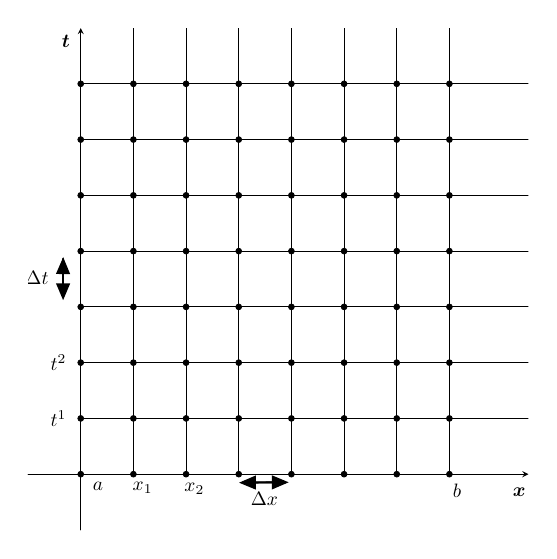
\begin{tikzpicture}[scale=0.7pt,line cap=round,line join=round,>=triangle  45,x=0.9555555555555555cm,y=1.011764705882353cm]
        \begin{axis}[
        x=0.9555555555555555cm,y=1.011764705882353cm,
        axis lines=middle,
        xmin=-1,
        xmax=8.5,
        ymin=-1,
        ymax=8.0,
        xtick={-0.0},
        ytick={-0.0},]
        \clip(-1.0,-1.0) rectangle (8.5,8.5);
        \draw (0.1,-0.01492590769987644) node[anchor=north west] {$a$};
        \draw (6.936006015235138,-0.04625816247894026) node[anchor=north west] {$b$};
        \draw (-1.18,3.765832835640491) node[anchor=north west] {$\Delta t$};
        \draw (3.1,-0.20291943637425935) node[anchor=north west] {$\Delta x$};
        \draw (0.8575485880967675,-0.01492590769987644) node[anchor=north west] {$x_1$};
        \draw (1.839292571174099,-0.03581407755258566) node[anchor=north west] {$x_2$};
        \draw (-0.7,1.2592524533153857) node[anchor=north west] {$t^1$};
        \draw (-0.7,2.2723286911717824) node[anchor=north west] {$t^2$};
        \draw (8.074411272207788,-0.12981084188977712) node[anchor=north west] {$\boldsymbol{x}$};
        \draw (-0.49,8) node[anchor=north west] {$\boldsymbol{t}$};
        \draw [->,line width=1.pt] (-0.3346034577059823,3.8604740672051325) -- (-0.3346034577059823,3.1204740672051328);
        \draw [->,line width=1.pt] (-0.3346034577059823,3.7017839952482134) -- (-0.3329059840463152,3.8906629755388313);
        \draw [->,line width=1.pt] (3.121531540966689,-0.14907205546295046) -- (3.948030184929092,-0.14559937208495718);
        \draw [->,line width=1.pt] (3.823001199491475,-0.1461247039565438) -- (3.0069329894929098,-0.15254473884094374);
        \draw [line width=0.5pt] (1.,0.) -- (1.,8.);
        \draw [line width=0.5pt] (2.,0.) -- (2.,8.);
        \draw [line width=0.5pt] (3.,0.) -- (3.,8.);
        \draw [line width=0.5pt] (4.,0.) -- (4.,8.);
        \draw [line width=0.5pt] (5.,0.) -- (5.,8.);
        \draw [line width=0.5pt] (6.,0.) -- (6.,8.);
        \draw [line width=0.5pt] (7.,0.) -- (7.,8.);
        \draw [line width=0.5pt,domain=0.0:8.5] plot(\x,{(--7.-0.*\x)/7.});
        \draw [line width=0.5pt,domain=0.0:8.5] plot(\x,{(--4.-0.*\x)/2.});
        \draw [line width=0.5pt,domain=0.0:8.5] plot(\x,{(--3.-0.*\x)/1.});
        \draw [line width=0.5pt,domain=0.0:8.5] plot(\x,{(--4.-0.*\x)/1.});
        \draw [line width=0.5pt,domain=0.0:8.5] plot(\x,{(--5.-0.*\x)/1.});
        \draw [line width=0.5pt,domain=0.0:8.5] plot(\x,{(--6.-0.*\x)/1.});
        \draw [line width=0.5pt,domain=0.0:8.5] plot(\x,{(--7.-0.*\x)/1.});
        \begin{scriptsize}
        \draw [fill=black] (1.,0.) circle (1.5pt);
        \draw [fill=black] (2.,0.) circle (1.5pt);
        \draw [fill=black] (3.,0.) circle (1.5pt);
        \draw [fill=black] (4.,0.) circle (1.5pt);
        \draw [fill=black] (5.,0.) circle (1.5pt);
        \draw [fill=black] (6.,0.) circle (1.5pt);
        \draw [fill=black] (7.,0.) circle (1.5pt);
        \draw [fill=black] (0.,0.) circle (1.5pt);
        \draw [fill=black] (0.,1.) circle (1.5pt);
        \draw [fill=black] (0.,2.) circle (1.5pt);
        \draw [fill=black] (0.,3.) circle (1.5pt);
        \draw [fill=black] (0.,4.) circle (1.5pt);
        \draw [fill=black] (0.,5.) circle (1.5pt);
        \draw [fill=black] (0.,6.) circle (1.5pt);
        \draw [fill=black] (0.,7.) circle (1.5pt);
        \draw [fill=black] (1.,1.) circle (1.5pt);
        \draw [fill=black] (1.,2.) circle (1.5pt);
        \draw [fill=black] (1.,3.) circle (1.5pt);
        \draw [fill=black] (1.,4.) circle (1.5pt);
        \draw [fill=black] (1.,5.) circle (1.5pt);
        \draw [fill=black] (1.,6.) circle (1.5pt);
        \draw [fill=black] (1.,7.) circle (1.5pt);
        \draw [fill=black] (2.,1.) circle (1.5pt);
        \draw [fill=black] (3.,1.) circle (1.5pt);
        \draw [fill=black] (4.,1.) circle (1.5pt);
        \draw [fill=black] (5.,1.) circle (1.5pt);
        \draw [fill=black] (6.,1.) circle (1.5pt);
        \draw [fill=black] (7.,1.) circle (1.5pt);
        \draw [fill=black] (2.,2.) circle (1.5pt);
        \draw [fill=black] (3.,2.) circle (1.5pt);
        \draw [fill=black] (4.,2.) circle (1.5pt);
        \draw [fill=black] (2.,3.) circle (1.5pt);
        \draw [fill=black] (2.,4.) circle (1.5pt);
        \draw [fill=black] (2.,5.) circle (1.5pt);
        \draw [fill=black] (2.,6.) circle (1.5pt);
        \draw [fill=black] (2.,7.) circle (1.5pt);
        \draw [fill=black] (3.,3.) circle (1.5pt);
        \draw [fill=black] (3.,4.) circle (1.5pt);
        \draw [fill=black] (3.,5.) circle (1.5pt);
        \draw [fill=black] (3.,6.) circle (1.5pt);
        \draw [fill=black] (3.,7.) circle (1.5pt);
        \draw [fill=black] (4.,3.) circle (1.5pt);
        \draw [fill=black] (4.,4.) circle (1.5pt);
        \draw [fill=black] (4.,5.) circle (1.5pt);
        \draw [fill=black] (4.,6.) circle (1.5pt);
        \draw [fill=black] (4.,7.) circle (1.5pt);
        \draw [fill=black] (5.,2.) circle (1.5pt);
        \draw [fill=black] (5.,3.) circle (1.5pt);
        \draw [fill=black] (5.,4.) circle (1.5pt);
        \draw [fill=black] (5.,5.) circle (1.5pt);
        \draw [fill=black] (5.,6.) circle (1.5pt);
        \draw [fill=black] (5.,7.) circle (1.5pt);
        \draw [fill=black] (6.,2.) circle (1.5pt);
        \draw [fill=black] (6.,3.) circle (1.5pt);
        \draw [fill=black] (6.,4.) circle (1.5pt);
        \draw [fill=black] (6.,5.) circle (1.5pt);
        \draw [fill=black] (6.,6.) circle (1.5pt);
        \draw [fill=black] (6.,7.) circle (1.5pt);
        \draw [fill=black] (7.,2.) circle (1.5pt);
        \draw [fill=black] (7.,3.) circle (1.5pt);
        \draw [fill=black] (7.,4.) circle (1.5pt);
        \draw [fill=black] (7.,5.) circle (1.5pt);
        \draw [fill=black] (7.,6.) circle (1.5pt);
        \draw [fill=black] (7.,7.) circle (1.5pt);
        \end{scriptsize}
        \end{axis}
        \end{tikzpicture}
    %\caption{}
    %\label{fig:my_label}
\end{figure}

\-\\\underline{Idea}: We'll impose $U_t(x_i,t^n) - U_{xx}(x_i,t^n) = f(x_i,t^n)$

\newpage

\subsubsection{Numerical derivatives}

\definecolor{qqwwzz}{rgb}{0.,0.4,0.6}

\begin{figure}[h]
    \centering
    \begin{tikzpicture}[line cap=round,line join=round,>=triangle 45,x=1.0cm,y=1.0cm]
    \begin{axis}[
    x=1.0cm,y=1.0cm,
    axis lines=middle,
    xmin=9.0,
    xmax=19.0,
    ymin=-1.0,
    ymax=7.0,
    xtick={0.0},
    ytick={0.0},y axis line style={draw = none}]
    \clip(9.,-1.) rectangle (19.,7.);
    \draw[line width=1.pt, smooth,samples=100,domain=0.0:0.11] plot[parametric] function{37.06*t**(3.0)+0.0*t**(2.0)+5.7*t+9.8,-38.54*t**(3.0)+0.0*t**(2.0)+7.51*t+3.02};
    \draw[line width=1.pt, smooth,samples=100,domain=0.11:0.15] plot[parametric] function{-52.47*t**(3.0)+28.91*t**(2.0)+2.59*t+9.91,39.61*t**(3.0)-25.24*t**(2.0)+10.22*t+2.92};
    \draw[line width=1.pt, smooth,samples=100,domain=0.15:0.24] plot[parametric] function{1.47*t**(3.0)+4.08*t**(2.0)+6.4*t+9.72,-18.89*t**(3.0)+1.69*t**(2.0)+6.09*t+3.13};
    \draw[line width=1.pt, smooth,samples=100,domain=0.24:0.3] plot[parametric] function{-13.11*t**(3.0)+14.44*t**(2.0)+3.95*t+9.91,9.63*t**(3.0)-18.57*t**(2.0)+10.89*t+2.76};
    \draw[line width=1.pt, smooth,samples=100,domain=0.3:0.35] plot[parametric] function{-7.62*t**(3.0)+9.58*t**(2.0)+5.38*t+9.77,-31.65*t**(3.0)+18.04*t**(2.0)+0.07*t+3.82};
    \draw[line width=1.pt, smooth,samples=100,domain=0.35:0.41] plot[parametric] function{-10.98*t**(3.0)+13.12*t**(2.0)+4.13*t+9.92,72.27*t**(3.0)-91.76*t**(2.0)+38.74*t-0.72};
    \draw[line width=1.pt, smooth,samples=100,domain=0.41:0.49] plot[parametric] function{3.59*t**(3.0)-4.8*t**(2.0)+11.48*t+8.91,47.73*t**(3.0)-61.58*t**(2.0)+26.37*t+0.97};
    \draw[line width=1.pt, smooth,samples=100,domain=0.49:0.57] plot[parametric] function{-20.86*t**(3.0)+30.92*t**(2.0)-5.91*t+11.73,40.31*t**(3.0)-50.75*t**(2.0)+21.09*t+1.83};
    \draw[line width=1.pt, smooth,samples=100,domain=0.57:0.62] plot[parametric] function{-10.43*t**(3.0)+13.18*t**(2.0)+4.14*t+9.84,-36.6*t**(3.0)+80.04*t**(2.0)-53.05*t+15.84};
    \draw[line width=1.pt, smooth,samples=100,domain=0.62:0.7] plot[parametric] function{28.35*t**(3.0)-59.13*t**(2.0)+49.1*t+0.52,-54.92*t**(3.0)+114.21*t**(2.0)-74.29*t+20.24};
    \draw[line width=1.pt, smooth,samples=100,domain=0.7:0.77] plot[parametric] function{-7.01*t**(3.0)+14.63*t**(2.0)-2.2*t+12.41,14.24*t**(3.0)-30.06*t**(2.0)+26.04*t-3.02};
    \draw[line width=1.pt, smooth,samples=100,domain=0.77:0.85] plot[parametric] function{36.51*t**(3.0)-85.69*t**(2.0)+74.89*t-7.34,-63.54*t**(3.0)+149.23*t**(2.0)-111.73*t+32.27};
    \draw[line width=1.pt, smooth,samples=100,domain=0.85:0.92] plot[parametric] function{-17.36*t**(3.0)+51.06*t**(2.0)-40.83*t+25.3,-8.72*t**(3.0)+10.06*t**(2.0)+6.03*t-0.95};
    \draw [line width=1.pt,dotted] (14.,0.)-- (13.99722993459645,4.732881120180119);
    \draw [line width=1.pt, >=latex, <->] (10.2,0.36)-- (13.6,0.36);
    \draw [line width=1.pt, >=latex, <->] (14.38,0.34)-- (17.88,0.34);
    \draw (11.76,1.06) node[anchor=north west] {$h$};
    \draw (15.9,1.04) node[anchor=north west] {$h$};
    \draw (9.52,0.) node[anchor=north west] {$x_{i-1}$};
    \draw (17.94,-0.04) node[anchor=north west] {$x_{i+1}$};
    \draw (13.84,0.) node[anchor=north west] {$x_{i}$};
    \draw (17.5,6.6) node[anchor=north west] {$f$};
    \draw (13,5.58) node[anchor=north west] {$f_i = f(x_i)$};
    \begin{scriptsize}
    \draw [color=qqwwzz] (14.,0.)-- ++(-1.5pt,0 pt) -- ++(3.0pt,0 pt) ++(-1.5pt,-1.5pt) -- ++(0 pt,3.0pt);
    \draw [fill=qqwwzz] (13.99722993459645,4.732881120180119) circle (1.5pt);
    \draw [color=black] (9.82,0.)-- ++(-1.5pt,0 pt) -- ++(3.0pt,0 pt) ++(-1.5pt,-1.5pt) -- ++(0 pt,3.0pt);
    \draw [color=black] (18.18,0.)-- ++(-1.5pt,0 pt) -- ++(3.0pt,0 pt) ++(-1.5pt,-1.5pt) -- ++(0 pt,3.0pt);
    \draw [fill=black,shift={(10.2,0.36)},rotate=90] (0,0) ++(0 pt,2.25pt) -- ++(1.9485571585149868pt,-3.375pt)--++(-3.8971143170299736pt,0 pt) -- ++(1.9485571585149868pt,3.375pt);
    \draw [fill=black,shift={(13.6,0.36)},rotate=270] (0,0) ++(0 pt,2.25pt) -- ++(1.9485571585149868pt,-3.375pt)--++(-3.8971143170299736pt,0 pt) -- ++(1.9485571585149868pt,3.375pt);
    \draw [fill=black,shift={(14.38,0.34)},rotate=90] (0,0) ++(0 pt,2.25pt) -- ++(1.9485571585149868pt,-3.375pt)--++(-3.8971143170299736pt,0 pt) -- ++(1.9485571585149868pt,3.375pt);
    \draw [fill=black,shift={(17.88,0.34)},rotate=270] (0,0) ++(0 pt,2.25pt) -- ++(1.9485571585149868pt,-3.375pt)--++(-3.8971143170299736pt,0 pt) -- ++(1.9485571585149868pt,3.375pt);
    \end{scriptsize}
    \end{axis}
    \end{tikzpicture}
    %\caption{}
    %\label{fig:my_label}
\end{figure}

We'll use Taylor's expansion on $f$ to find an approximation for the derivatives:
\begin{enumerate}[label={(\arabic*)}]
    \item $f_{i+1} = f_i + hf_i' + \frac{h^2}{2}f_i'' + \frac{h^3}{3!}f_i''' + \ldots$
    \item $f_{i-1} = f_i - hf_i' + \frac{h^2}{2}f_i'' - \frac{h^3}{3!}f_i''' + \ldots$
\end{enumerate}\-\\

\underline{Approximation of the first derivative}: \\
\begin{itemize}
    \item Forward differences (1) $$f_i' = \frac{f_{i+1} - f_i}{h} + \mathcal{O}(h)$$
    \item Backwards differences (2) $$f_i' = \frac{f_i-f_{i-1}}{h} + \mathcal{O}(h)$$
    \item Centered differences (1)-(2) $$f_i' = \frac{f_{i+1} - f_{i-1}}{2h} + \mathcal{O}(h^2)$$
\end{itemize}

\begin{remark}
  With centered differences, it converges faster, but sometimes the other two methods are preferable for ease in computations.
\end{remark}

\underline{Approximation of the second derivative} (1)+(2) $$f_i'' = \frac{f_{i+1} - 2f_i + f_{i-1}}{h^2} + \mathcal{O}(h^2)$$\\

There are higher order approximations, but these are the standard, and are more than enough. \\

Now, we'll present some notation to differentiate between the problem we want to solve and the numerical problem.

\begin{definition}\-\\
  The \textbf{continuous problem} is 
  $
    \begin{cases}
      \mathcal{L}(u) = f &\text{ in } \Omega, \, t > 0 \\
      \mathcal{B}(u) = q &\text{ in } \partial \Omega, t > 0 \\
      u(x,0) = u_0(x)
    \end{cases}
  $\\
  
  \-\\Where $\mathcal{L}$ is any differential operator. \\
  
  It's what we want to solve. \\
  
  The \textbf{discrete problem} \hspace{0.08cm}is\hspace{0.3cm}
  $
    \begin{cases}
      L(u) + \tau = f \\
      B(u) + \overline{\tau} = q \\
      u(x,0) = u_0(x)
    \end{cases}
  $\\
  
  \-\\The \textbf{numerical problem} is
  $
    \begin{cases}
      L(U) = f \\
      B(U) = q \\
      U(x,0) = u_0(x)
    \end{cases}
  $
\end{definition}

\-\\

Let's go back to our 1D heat equation: \\

The continuous problem is 

\[
\begin{cases}
  u_t - u_{xx} = f \quad t>0, x\in(a,b)\\
  u(a,t) = u_a\\
  u(b,t) = u_b \\
  u(x,0) = u_0(x)
\end{cases}
\]

\underline{Notation}: $u(x_i,t^n) = u_i^n$ \\
$x_i = a + i\Delta x \quad i = 0,\ldots N \quad x_0 = a,\, x_N = b \qquad$ (sometimes $\Delta x = h$).\\
$t^n = n\Delta t \, n\geq0$\\

\newpage

We have the following explicit method:

\subsubsection{Forward Time Centered Space method (FTCS)}

\begin{itemize}
    \item Approximate $u_t$ using forward differences (FT)
    \item Approximate $u_{xx}$ using centered differences (CD)
\end{itemize}

Our discretized problem is

\[
  \frac{u_i^{n+1} - u_i^n}{\Delta t} + \bigo(\Delta t) - \frac{u_{i+1}^n - 2u_i^n + u_{i-1}^n}{\Delta x^2} + \bigo(\Delta x^2) = f_i^n
\]

We define $\tau = \bigo(\Delta t,\Delta x^2)$ \\

Neglecting $\tau$, the numerical problem we want to solve is

\[
  \begin{cases}
    \dfrac{U_i^{n+1} - U_i^n}{\Delta t} - \dfrac{U_{i+1}^n - 2U_i^n + U_{i-1}^n}{\Delta x^2} = f_i^n \vspace{0.2cm}\\
    U_0^{n+1} = u_a(t^{n+1})\\
    U_N^{n+1} = u_b(t^{n+1}) \\
    U_i^0 = u_0(x_i)
  \end{cases}
\]

Now we define $r$ as $$r = \frac{\Delta t}{\Delta x^2}$$

So $$U_i^{n+1} = rU_{i-1}^n + (1-2r)U_i^n + rU_{i+1}^n + \Delta t f_i^n \qquad i = 1,\ldots,N-1$$

For $i=1$, $$U_1^{n+1} = (1-2r)U_1^n + rU_2^n + \Delta t f_1^n + ru_a^n$$

And for $i=N-1$, $$U_{N-1}^{n+1} = rU_{N-2}^n + (1-2r)U_{N-1}^n + \Delta t f_{N-1}^n + ru_b^n$$

Thus, $$\overline{U^{n+1}} = \underset{^\sim}{B}\overline{U^n} + \overline{F} + \overline{G}$$

Where 

$$\overline{U^p} = \left(U_1^p, U_2^p, \ldots , U_{N-1}^p \right)^T \qquad \overline{F}=\Delta t\left(f_1^n, f_2^n, \ldots,f_{N-1}^n \right)^T \qquad \overline{G} = \left(ru_a^n, 0, \ldots,0,ru_b^n \right)^T$$
$$
  \underset{^\sim}{B} = 
  \begin{pmatrix}
    \scriptstyle\small{1-2r} & r \\
    r    & \scriptstyle\small{1-2r} & r \\
         & \ddots & \ddots & \ddots \\
         &        & r & \scriptstyle\small{1-2r} & r \\
         &        &   & r    & \scriptstyle\small{1-2r}
  \end{pmatrix}
$$

\newpage

$\ldots$

\newpage
\section{Numerical Solution of PDEs with the Finite Elements Method}

\subsection{From the strong form to the weak form}

Given the following problem in \textbf{strong form}: 

\[
  \begin{cases}
    \nabla\cdot\left(\subTilde{A}\,\nabla u\right) = -s \quad &\text{in }\Omega\\
    u = u_D \quad &\text{on } \Gamma_D\\
    \subTilde{A}\frac{\partial u}{\partial n} = q \quad &\text{on } \Gamma_N
  \end{cases}
\]

Where 
\begin{align*}
      \Gamma_D\cup\Gamma_N &= \partial\Omega\\
      \Gamma_D\cap\Gamma_N &= \varnothing
\end{align*}

$s$ is the source term (it's a function), but for the moment we'll assume that both $s$ and $\subTilde{A}$ don't depend on $u$. \\

We'll derive the equivalent weak form of the problem using \textbf{weighted residuals}:

\[
  \int_\Omega\omega\nabla\cdot\left(\subTilde{A}\,\nabla u\right)\,d\Omega = -\int_\Omega \omega s \, d\Omega \qquad\forall \omega \text{ such that } \omega = 0 \text{ on } \Gamma_D
\]

Where $\omega$ is the \textbf{test function} (or \textbf{weighting function}). \\

We integrate by parts:

\[
  -\int_{\Omega} \nabla\omega\cdot\left(\subTilde{A}\,\nabla u\right)\,d\Omega + \int_{\partial\Omega} \omega\subTilde{A}\nabla u\cdot\Bar{n} \,d\Gamma = -\int_\Omega \omega s \, d\Omega
\]\-\\
Let's have a look at the term on $\partial\Omega$

\[
  \int_{\partial\Omega} \omega\subTilde{A}\nabla u\cdot\Bar{n} \,d\Gamma = \int_{\Gamma_D} \cancelto{^{\footnotesize{\scriptstyle{0} \text{ (by def)}}}}{\omega} \hspace{-1.2cm}\subTilde{A}\nabla u\cdot\Bar{n} \,d\Gamma + \int_{\Gamma_N} \omega\underbrace{\subTilde{A}\nabla u\cdot\Bar{n}}_{q} \,d\Gamma = \int_{\Gamma_N} \omega q \, d\Gamma
\]

And with that, we get \\

\underline{\textbf{Weak form}} \\

We have to find $u$ such that $u = u_D$ on $\Gamma_D$ and 

\[
  \int_{\Omega} \nabla\omega\cdot\left(\subTilde{A}\,\nabla u\right)\,d\Omega = \int_\Omega \omega s \, d\Omega + \int_{\Gamma_N} \omega q \, d\Gamma \qquad \forall \omega \text{ such that } \omega = 0 \text{ on } \Gamma_D
\]
\newpage

So $$u \in \mathcal{H}_{\Gamma_D}^1(\Omega) = \setb{u\in\mathcal{H}^1(\Omega)\, \big| \, u=u_D \text{ on } \Gamma_D}$$

and $$\omega \in \mathcal{H}_{\Gamma_D,0}^1(\Omega) = \setb{u \in \mathcal{H}^1(\Omega) \,\big| \, u = 0 \text{ on } \Gamma_D}$$ \-\\
Where $$\mathcal{H}^1(\Omega) = \setb{f\in L^2(\Omega)\, \big| \, \frac{\partial f}{\partial x_i}\in L^2(\Omega)\quad \forall i} \qquad L^2(\Omega) = \setb{f \, \big| \, \int_{\Omega} f^2\,d\Omega < \infty}$$\-\\

Now that we have the weak form, what we do is discretize the domain.

\subsection{Discretisation}

The mesh is defined by a set of points and triangles like:

\begin{figure}[h]
    \centering
    \definecolor{xdxdff}{rgb}{0.49019607843137253,0.49019607843137253,1.}
\definecolor{ududff}{rgb}{0.30196078431372547,0.30196078431372547,1.}
\begin{tikzpicture}[line cap=round,line join=round,>=triangle 45,x=1.0cm,y=1.0cm]
\clip(1.6,-3.5) rectangle (12.9,2.7);
\draw[line width=1.pt, smooth,samples=100,domain=0.0:0.12] plot[parametric] function{75.25*t**(3.0)+0.0*t**(2.0)+7.52*t+2.02,-84.83*t**(3.0)+0.0*t**(2.0)+10.33*t+0.64};
\draw[line width=1.pt, smooth,samples=100,domain=0.12:0.24] plot[parametric] function{-96.18*t**(3.0)+59.18*t**(2.0)+0.71*t+2.28,-35.0*t**(3.0)-17.2*t**(2.0)+12.31*t+0.56};
\draw[line width=1.pt, smooth,samples=100,domain=0.24:0.34] plot[parametric] function{-2.71*t**(3.0)-8.78*t**(2.0)+17.18*t+0.95,112.71*t**(3.0)-124.59*t**(2.0)+38.34*t-1.54};
\draw[line width=1.pt, smooth,samples=100,domain=0.34:0.41] plot[parametric] function{79.9*t**(3.0)-91.82*t**(2.0)+45.01*t-2.16,75.81*t**(3.0)-87.5*t**(2.0)+25.91*t-0.15};
\draw[line width=1.pt, smooth,samples=100,domain=0.41:0.5] plot[parametric] function{13.49*t**(3.0)-9.87*t**(2.0)+11.3*t+2.46,70.33*t**(3.0)-80.73*t**(2.0)+23.13*t+0.23};
\draw[line width=1.pt, smooth,samples=100,domain=0.5:0.56] plot[parametric] function{-51.11*t**(3.0)+87.16*t**(2.0)-37.28*t+10.57,-94.01*t**(3.0)+166.12*t**(2.0)-100.47*t+20.86};
\draw[line width=1.pt, smooth,samples=100,domain=0.56:0.64] plot[parametric] function{-1.28*t**(3.0)+3.34*t**(2.0)+9.71*t+1.79,-8.34*t**(3.0)+22.01*t**(2.0)-19.67*t+5.76};
\draw[line width=1.pt, smooth,samples=100,domain=0.64:0.72] plot[parametric] function{-0.48*t**(3.0)+1.79*t**(2.0)+10.71*t+1.58,3.42*t**(3.0)-0.57*t**(2.0)-5.21*t+2.67};
\draw[line width=1.pt, smooth,samples=100,domain=0.72:0.8] plot[parametric] function{-20.09*t**(3.0)+44.27*t**(2.0)-19.95*t+8.95,-166.5*t**(3.0)+367.38*t**(2.0)-270.81*t+66.58};
\draw[line width=1.pt, smooth,samples=100,domain=0.8:0.85] plot[parametric] function{-120.37*t**(3.0)+283.57*t**(2.0)-210.3*t+59.42,-105.76*t**(3.0)+222.45*t**(2.0)-155.53*t+36.01};
\draw[line width=1.pt, smooth,samples=100,domain=0.85:0.94] plot[parametric] function{-143.65*t**(3.0)+343.17*t**(2.0)-261.17*t+73.89,143.87*t**(3.0)-416.7*t**(2.0)+389.96*t-119.17};
\draw[line width=1.pt, smooth,samples=100,domain=0.0:0.07] plot[parametric] function{393.9*t**(3.0)+0.0*t**(2.0)-2.67*t+2.02,67.04*t**(3.0)+0.0*t**(2.0)-12.5*t+0.64};
\draw[line width=1.pt, smooth,samples=100,domain=0.07:0.13] plot[parametric] function{-337.89*t**(3.0)+147.54*t**(2.0)-12.59*t+2.24,68.66*t**(3.0)-0.33*t**(2.0)-12.48*t+0.64};
\draw[line width=1.pt, smooth,samples=100,domain=0.13:0.21] plot[parametric] function{-43.7*t**(3.0)+34.53*t**(2.0)+1.88*t+1.62,-53.54*t**(3.0)+46.61*t**(2.0)-18.49*t+0.9};
\draw[line width=1.pt, smooth,samples=100,domain=0.21:0.31] plot[parametric] function{-21.13*t**(3.0)+20.17*t**(2.0)+4.93*t+1.41,-46.39*t**(3.0)+42.06*t**(2.0)-17.53*t+0.83};
\draw[line width=1.pt, smooth,samples=100,domain=0.31:0.44] plot[parametric] function{10.17*t**(3.0)-9.22*t**(2.0)+14.13*t+0.45,60.42*t**(3.0)-58.23*t**(2.0)+13.86*t-2.45};
\draw[line width=1.pt, smooth,samples=100,domain=0.44:0.56] plot[parametric] function{-16.23*t**(3.0)+25.85*t**(2.0)-1.4*t+2.74,-67.07*t**(3.0)+111.11*t**(2.0)-61.11*t+8.62};
\draw[line width=1.pt, smooth,samples=100,domain=0.56:0.68] plot[parametric] function{6.95*t**(3.0)-12.91*t**(2.0)+20.2*t-1.27,3.67*t**(3.0)-7.16*t**(2.0)+4.8*t-3.63};
\draw[line width=1.pt, smooth,samples=100,domain=0.68:0.77] plot[parametric] function{-17.33*t**(3.0)+36.26*t**(2.0)-12.99*t+6.2,-45.12*t**(3.0)+91.66*t**(2.0)-61.9*t+11.38};
\draw[line width=1.pt, smooth,samples=100,domain=0.77:0.86] plot[parametric] function{50.85*t**(3.0)-120.86*t**(2.0)+107.71*t-24.71,72.61*t**(3.0)-179.67*t**(2.0)+146.53*t-41.99};
\draw[line width=1.pt, smooth,samples=100,domain=0.86:0.94] plot[parametric] function{-229.77*t**(3.0)+604.9*t**(2.0)-517.97*t+155.09,319.02*t**(3.0)-816.96*t**(2.0)+695.94*t-199.87};
\draw [line width=1.pt] (3.,1.7)-- (3.42,0.46);
\draw [line width=1.pt] (2.02,0.64)-- (3.42,0.46);
\draw [line width=1.pt] (3.42,0.46)-- (1.96,-0.18);
\draw [line width=1.pt] (3.42,0.46)-- (2.34,-0.82);
\draw [line width=1.pt] (3.42,0.46)-- (3.74,-0.78);
\draw [line width=1.pt] (3.74,-0.78)-- (2.34,-0.82);
\draw [line width=1.pt] (3.74,-0.78)-- (3.16,-1.44);
\draw [line width=1.pt] (3.42,0.46)-- (4.04,1.2);
\draw [line width=1.pt] (3.,1.7)-- (4.04,1.2);
\draw [line width=1.pt] (3.,1.7)-- (2.4942912053784743,1.249476159149053);
\draw [line width=1.pt] (2.4942912053784743,1.249476159149053)-- (3.42,0.46);
\draw [line width=1.pt] (3.,1.7)-- (3.712654741773794,2.0071982078016495);
\draw [line width=1.pt] (3.712654741773794,2.0071982078016495)-- (4.04,1.2);
\draw [line width=1.pt] (4.56,2.04)-- (4.04,1.2);
\draw [line width=1.pt] (4.04,1.2)-- (4.56,0.08);
\draw [line width=1.pt] (4.56,0.08)-- (3.42,0.46);
\draw [line width=1.pt] (3.74,-0.78)-- (4.56,0.08);
\draw [line width=1.pt] (4.56,0.08)-- (4.8,-1.18);
\draw [line width=1.pt] (4.8,-1.18)-- (3.74,-0.78);
\draw [line width=1.pt] (3.74,-0.78)-- (4.28,-1.96);
\draw [line width=1.pt] (4.28,-1.96)-- (4.8,-1.18);
\draw [line width=1.pt] (4.56,0.08)-- (5.14,0.74);
\draw [line width=1.pt] (4.04,1.2)-- (5.14,0.74);
\draw [line width=1.pt] (5.14,0.74)-- (4.56,2.04);
\draw [line width=1.pt] (5.14,0.74)-- (5.62,1.56);
\draw [line width=1.pt] (5.14,0.74)-- (6.38,0.98);
\draw [line width=1.pt] (6.38,0.98)-- (5.84,-0.04);
\draw [line width=1.pt] (5.84,-0.04)-- (5.14,0.74);
\draw [line width=1.pt] (4.56,0.08)-- (5.84,-0.04);
\draw [line width=1.pt] (5.84,-0.04)-- (4.8,-1.18);
\draw [line width=1.pt] (4.8,-1.18)-- (5.113955707955139,-2.29710660508585);
\draw [line width=1.pt] (5.113955707955139,-2.29710660508585)-- (5.88,-1.66);
\draw [line width=1.pt] (4.8,-1.18)-- (5.88,-1.66);
\draw [line width=1.pt] (5.88,-1.66)-- (5.84,-0.04);
\draw [line width=1.pt] (5.84,-0.04)-- (6.825974218356539,0.669567582001636);
\draw [line width=1.pt] (6.825974218356539,0.669567582001636)-- (6.72,-0.44);
\draw [line width=1.pt] (6.72,-0.44)-- (5.84,-0.04);
\draw [line width=1.pt] (5.88,-1.66)-- (6.72,-0.44);
\draw [line width=1.pt] (5.88,-1.66)-- (5.78,-2.48);
\draw [line width=1.pt] (5.78,-2.48)-- (6.62,-1.82);
\draw [line width=1.pt] (6.62,-1.82)-- (6.439881234920367,-2.543484329382041);
\draw [line width=1.pt] (6.62,-1.82)-- (5.88,-1.66);
\draw [line width=1.pt] (6.62,-1.82)-- (6.72,-0.44);
\draw [line width=1.pt] (6.72,-0.44)-- (7.34,0.4);
\draw [line width=1.pt] (6.72,-0.44)-- (7.7,-0.82);
\draw [line width=1.pt] (7.7,-0.82)-- (7.34,0.4);
\draw [line width=1.pt] (7.7,-0.82)-- (8.06,0.18);
\draw [line width=1.pt] (7.7,-0.82)-- (9.04,0.);
\draw [line width=1.pt] (6.62,-1.82)-- (7.7,-0.82);
\draw [line width=1.pt] (6.62,-1.82)-- (7.18,-2.54);
\draw [line width=1.pt] (7.18,-2.54)-- (7.7,-0.82);
\draw [line width=1.pt] (7.7,-0.82)-- (8.62,-2.52);
\draw [line width=1.pt] (7.8,-1.86)-- (7.18,-2.54);
\draw [line width=1.pt] (7.8,-1.86)-- (8.62,-2.52);
\draw [line width=1.pt] (7.8,-1.86)-- (7.7,-0.82);
\draw [line width=1.pt] (9.04,0.)-- (8.76,-1.14);
\draw [line width=1.pt] (8.76,-1.14)-- (7.7,-0.82);
\draw [line width=1.pt] (8.76,-1.14)-- (8.62,-2.52);
\draw [line width=1.pt] (8.76,-1.14)-- (9.76,-2.54);
\draw [line width=1.pt] (9.76,-2.54)-- (9.58,-1.32);
\draw [line width=1.pt] (9.58,-1.32)-- (8.76,-1.14);
\draw [line width=1.pt] (5.092888033673837,1.8678505213242278)-- (5.14,0.74);
\draw [line width=1.pt] (4.0628882464444835,2.0625098738473846)-- (4.04,1.2);
\draw [line width=1.pt] (1.9491558597261478,0.2563349465687549)-- (3.42,0.46);
\draw [line width=1.pt] (2.0989776852520947,-0.5084240269385761)-- (3.42,0.46);
\draw [line width=1.pt] (2.7145919118495003,-1.1537811154633195)-- (3.74,-0.78);
\draw [line width=1.pt] (9.58,-1.32)-- (9.04,0.);
\draw [line width=1.pt] (9.58,-1.32)-- (10.06,-0.1);
\draw [line width=1.pt] (10.06,-0.1)-- (10.54,-1.1);
\draw [line width=1.pt] (10.54,-1.1)-- (9.58,-1.32);
\draw [line width=1.pt] (10.54,-1.1)-- (10.98,-0.18);
\draw [line width=1.pt] (10.54,-1.1)-- (11.66,-0.44);
\draw [line width=1.pt] (11.286580727568996,-0.2608506072605792)-- (10.54,-1.1);
\draw [line width=1.pt] (10.54,-1.1)-- (9.76,-2.54);
\draw [line width=1.pt] (10.54,-1.1)-- (10.9,-2.68);
\draw [line width=1.pt] (10.9,-2.68)-- (11.28,-1.44);
\draw [line width=1.pt] (11.28,-1.44)-- (10.54,-1.1);
\draw [line width=1.pt] (11.66,-0.44)-- (11.28,-1.44);
\draw [line width=1.pt] (11.28,-1.44)-- (12.033119901892462,-0.7777540285797073);
\draw [line width=1.pt] (12.3,-1.28)-- (11.28,-1.44);
\draw [line width=1.pt] (11.82,-2.6)-- (11.28,-1.44);
\draw [line width=1.pt] (12.36,-2.06)-- (11.28,-1.44);
\draw [line width=1.pt] (12.36,-2.06)-- (11.82,-2.6);
\draw [line width=1.pt] (12.36,-2.06)-- (12.3,-1.28);
\draw [line width=1.pt] (11.379210153953807,-2.703128564449173)-- (11.28,-1.44);
\draw [line width=1.pt] (10.307753337995514,-2.6033413516884565)-- (10.54,-1.1);
\draw [line width=1.pt] (9.120009503922319,-2.5164145643048688)-- (8.76,-1.14);
\begin{scriptsize}
\draw [fill=ududff] (2.02,0.64) circle (2.5pt);
\draw [fill=ududff] (3.,1.7) circle (2.5pt);
\draw [fill=ududff] (4.56,2.04) circle (2.5pt);
\draw [fill=ududff] (5.62,1.56) circle (2.5pt);
\draw [fill=ududff] (6.38,0.98) circle (2.5pt);
\draw [fill=ududff] (7.34,0.4) circle (2.5pt);
\draw [fill=ududff] (8.06,0.18) circle (2.5pt);
\draw [fill=ududff] (9.04,0.) circle (2.5pt);
\draw [fill=ududff] (10.06,-0.1) circle (2.5pt);
\draw [fill=ududff] (10.98,-0.18) circle (2.5pt);
\draw [fill=ududff] (11.66,-0.44) circle (2.5pt);
\draw [fill=ududff] (12.3,-1.28) circle (2.5pt);
\draw [fill=ududff] (12.36,-2.06) circle (2.5pt);
\draw [fill=ududff] (1.96,-0.18) circle (2.5pt);
\draw [fill=ududff] (2.34,-0.82) circle (2.5pt);
\draw [fill=ududff] (3.16,-1.44) circle (2.5pt);
\draw [fill=ududff] (4.28,-1.96) circle (2.5pt);
\draw [fill=ududff] (5.78,-2.48) circle (2.5pt);
\draw [fill=ududff] (7.18,-2.54) circle (2.5pt);
\draw [fill=ududff] (8.62,-2.52) circle (2.5pt);
\draw [fill=ududff] (9.76,-2.54) circle (2.5pt);
\draw [fill=ududff] (10.9,-2.68) circle (2.5pt);
\draw [fill=ududff] (11.82,-2.6) circle (2.5pt);
\draw [fill=ududff] (3.42,0.46) circle (2.5pt);
\draw [fill=ududff] (3.74,-0.78) circle (2.5pt);
\draw [fill=ududff] (4.04,1.2) circle (2.5pt);
\draw [fill=xdxdff] (2.4942912053784743,1.249476159149053) circle (2.5pt);
\draw [fill=xdxdff] (3.712654741773794,2.0071982078016495) circle (2.5pt);
\draw [fill=ududff] (4.56,0.08) circle (2.5pt);
\draw [fill=ududff] (4.8,-1.18) circle (2.5pt);
\draw [fill=ududff] (5.14,0.74) circle (2.5pt);
\draw [fill=ududff] (5.84,-0.04) circle (2.5pt);
\draw [fill=xdxdff] (5.113955707955139,-2.29710660508585) circle (2.5pt);
\draw [fill=ududff] (5.88,-1.66) circle (2.5pt);
\draw [fill=xdxdff] (6.825974218356539,0.669567582001636) circle (2.5pt);
\draw [fill=ududff] (6.72,-0.44) circle (2.5pt);
\draw [fill=ududff] (6.62,-1.82) circle (2.5pt);
\draw [fill=xdxdff] (6.439881234920367,-2.543484329382041) circle (2.5pt);
\draw [fill=ududff] (7.7,-0.82) circle (2.5pt);
\draw [fill=ududff] (7.8,-1.86) circle (2.5pt);
\draw [fill=ududff] (8.76,-1.14) circle (2.5pt);
\draw [fill=ududff] (9.58,-1.32) circle (2.5pt);
\draw [fill=xdxdff] (5.092888033673837,1.8678505213242278) circle (2.5pt);
\draw [fill=xdxdff] (4.0628882464444835,2.0625098738473846) circle (2.5pt);
\draw [fill=xdxdff] (1.9491558597261478,0.2563349465687549) circle (2.5pt);
\draw [fill=xdxdff] (2.0989776852520947,-0.5084240269385761) circle (2.5pt);
\draw [fill=xdxdff] (2.7145919118495003,-1.1537811154633195) circle (2.5pt);
\draw [fill=ududff] (10.54,-1.1) circle (2.5pt);
\draw [fill=xdxdff] (11.286580727568996,-0.2608506072605792) circle (2.5pt);
\draw [fill=ududff] (11.28,-1.44) circle (2.5pt);
\draw [fill=xdxdff] (12.033119901892462,-0.7777540285797073) circle (2.5pt);
\draw [fill=xdxdff] (11.379210153953807,-2.703128564449173) circle (2.5pt);
\draw [fill=xdxdff] (10.307753337995514,-2.6033413516884565) circle (2.5pt);
\draw [fill=xdxdff] (9.120009503922319,-2.5164145643048688) circle (2.5pt);
\end{scriptsize}
\end{tikzpicture}
\caption{Mesh of a domain $\Omega$}
    \label{fig:mesh}
\end{figure}

We want the nodal values of the solution noted $u_i$ ($i = 1,\ldots,n_{\text{nodes}}$).\\

We'll approximate the solution $u$ by:

\[
  u \simeq \sum_i N_i(x)u_i
\]
\begin{definition}
  We define the \textbf{shape function} $N_i(x)$ as
  \[
    N_i(x_j) = \delta_{ij} = \begin{cases} 1 \text{ if } i=j \\ 0 \text{ otherwise} \end{cases}
  \]
  where $x_i$ is a node on the mesh.
  \begin{figure}
      \centering
      \definecolor{qqwwzz}{rgb}{0.,0.4,0.6}
      \begin{tikzpicture}[line cap=round,line join=round,>=triangle 45,x=1.0cm,y=1.0cm,scale=1.5]
        \clip(6.,-3.) rectangle (12.141,-0.5);
        \draw [line width=1.pt,domain=6.:12.141] plot(\x,{(-32.832-0.*\x)/13.68});
        \draw [line width=1.pt,color=qqwwzz] (6.02,-2.4)-- (7.72,-2.4);
        \draw [line width=1.pt,color=qqwwzz] (7.72,-2.4)-- (9.18,-1.);
        \draw [line width=1.pt,color=qqwwzz] (9.18,-1.)-- (10.66,-2.4);
        \draw [line width=1.pt,color=qqwwzz] (10.66,-2.4)-- (12.1,-2.4);
        \draw (8.9,-2.44) node[anchor=north west] {$x_i$};
        \draw (9.8,-1.1) node[anchor=north west] {$N_i$};
        \begin{scriptsize}
        \draw [color=black] (6.02,-2.4)-- ++(-2.0pt,0 pt) -- ++(4.0pt,0 pt) ++(-2.0pt,-2.0pt) -- ++(0 pt,4.0pt);
        \draw [color=black] (7.72,-2.4)-- ++(-2.0pt,0 pt) -- ++(4.0pt,0 pt) ++(-2.0pt,-2.0pt) -- ++(0 pt,4.0pt);
        \draw [color=black] (9.18,-2.4)-- ++(-2.0pt,0 pt) -- ++(4.0pt,0 pt) ++(-2.0pt,-2.0pt) -- ++(0 pt,4.0pt);
        \draw [color=black] (10.66,-2.4)-- ++(-2.0pt,0 pt) -- ++(4.0pt,0 pt) ++(-2.0pt,-2.0pt) -- ++(0 pt,4.0pt);
        \draw [color=black] (12.1,-2.4)-- ++(-2.0pt,0 pt) -- ++(4.0pt,0 pt) ++(-2.0pt,-2.0pt) -- ++(0 pt,4.0pt);
        \draw [fill=black] (9.18,-1.) circle (1.0pt);
        \end{scriptsize}
      \end{tikzpicture}
      \caption{$N_i$ are piecewise polynomials with compact support}
      \label{fig:Ni}
  \end{figure}
\end{definition}

Previously, we had to choose $\omega$ as the weighting function. The common approach is with the \textit{Galerkin approximation}: $$\omega = N_i \qquad i = 1,\ldots,n_{\text{nodes}}$$

For every $\omega$ chosen, we have an equation, so we choose as many $\omega$'s as unknowns. \\

Then 
\[
  \int_\Omega \nabla N_i \cdot \subTilde{A}\left(\sum_j\nabla N_ju_j\right)\,d\Omega = \int_\Omega N_is\,d\Omega + \int_{\Gamma_N}N_iq\,d\Gamma
\]
\[
  \sum_j\underbrace{\int_\Omega\left(\nabla N_i\cdot\subTilde{A}\nabla N_j\right)}_{K_{ij}}\,d\Omega \,\, u_j = \underbrace{\int_\Omega N_is\,d\Omega + \int_{\Gamma_N}N_iq\,d\Gamma}_{f_i}
\]

So we end up with the system

\[
  \sum_jK_{ij}u_j = f_i \qquad i=1,\ldots,n_{\text{nodes}}
\]

and in matrix form
\[
  \subTilde{K}\Bar{u} = \bar{f}
\]\-\\
$\subTilde{K}$ is singular, so we need to impose the Dirichlet conditions:

\[
  \sum_{j=1}^{n_{\text{nodes}}} N_j(x)u_j = \sum_{j\in U}N_j(x)u_j + \sum_{j\in D}N_j(x)u_j \qquad (u_j=u_D(x_j))
\]

where $\begin{cases}
    j\in D \text{ if } x_j \in \Gamma_D\\ j\in U \text{ if } x_j\not\in \Gamma_D
\end{cases}$

\newpage

\begin{example}
We'll work with the following 1D problem:
\[
  \begin{cases}
    -u_{xx} = f \\
    u(0) = 0, \, u(1) = 1
  \end{cases}
\]

with 
  \begin{figure}[h]
      \centering
      \definecolor{yqyqyq}{rgb}{0.5019607843137255,0.5019607843137255,0.5019607843137255}
        \definecolor{qqqqtt}{rgb}{0.,0.,0.2}
        \definecolor{qqttzz}{rgb}{0.,0.2,0.6}
        \definecolor{qqwwzz}{rgb}{0.,0.4,0.6}
        \begin{tikzpicture}[line cap=round,line join=round,>=triangle 45,x=12.0cm,y=4.8cm, scale = 0.8]
        \begin{axis}[
        x=12.0cm,y=4.8cm,
        axis lines=middle,
        xmin=-0.05,
        xmax=1.02,
        ymin=-0.2,
        ymax=1.12,
        xtick={-0.0,0.1,...,1.1},
        ytick={-0.0,1.0,...,1.0},]
        \clip(-0.05,-0.2) rectangle (1.02,1.12);
        \draw (0.17342001878856841,1.12) node[anchor=north west] {$N_1$};
        \draw (0.37535408033237305,1.12) node[anchor=north west] {$N_2$};
        \draw (0.6716703662933907,1.12) node[anchor=north west] {$N_3$};
        \draw (0.9306727495778357,1.12) node[anchor=north west] {$\psi$};
        \draw (-0.04826846181930405,-0.010428039332540924) node[anchor=north west] {$x_0$};
        \draw (0.175,-0.12) node[anchor=north west] {$x_1$};
        \draw (0.375,-0.12) node[anchor=north west] {$x_2$};
        \draw (0.675,-0.12) node[anchor=north west] {$x_3$};
        \draw (0.975,-0.12) node[anchor=north west] {$x_4$};
        \draw [line width=1.pt,color=qqwwzz] (-2.501762441637411E-4,0.)-- (0.1993279293434915,0.9966396467174575);
        \draw [line width=1.pt,color=qqwwzz] (0.1993279293434915,0.9966396467174575)-- (0.39890603493114674,0.);
        \draw [line width=1.pt,color=qqttzz] (0.1993279293434915,0.)-- (0.40112356943767624,0.9962547685410791);
        \draw [line width=1.pt,color=qqttzz] (0.40112356943767624,0.9962547685410791)-- (0.7004907278191591,0.0016357593971971784);
        \draw [line width=1.pt,color=qqttzz] (0.7004907278191591,0.0016357593971971784)-- (1.0508611798508205,0.);
        \draw [line width=1.pt,color=qqwwzz] (0.39890603493114674,0.)-- (0.7001812029617619,0.0026641263985551777);
        \draw [line width=1.pt,color=qqqqtt] (0.6982731933126296,0.9942439777087653)-- (0.3987606852809381,7.258372535798863E-4);
        \draw [line width=1.pt,color=qqqqtt] (0.6982731933126296,0.9942439777087653)-- (1,2.588335028239439E-4);
        \draw [line width=1.pt,color=qqqqtt] (0.3985896937652761,0.0015797231207659995)-- (-0.0556885389074013,0.);
        \draw [line width=1.pt,color=yqyqyq] (0.7003484276096387,0.0021085383558490656)-- (1.0222763403956587,1.0742544679855293);
        \draw [<->,line width=0.5 pt] (0.025,0.05) -- (0.19,0.05);
        \draw [<->,line width=0.5 pt] (0.22,0.05) -- (0.38,0.05);
        \draw [<->,line width=0.5 pt] (0.42,0.05) -- (0.68,0.05);
        \draw [<->,line width=0.5 pt] (0.72,0.05) -- (0.98,0.05);
        \draw (0.11,0.17) node[anchor=north] {$h_1$};
        \draw (0.3,0.17) node[anchor=north] {$h_2$};
        \draw (0.55,0.17) node[anchor=north] {$h_3$};
        \draw (0.85,0.17) node[anchor=north] {$h_4$};
        \end{axis}
        \end{tikzpicture}
      \caption{}
      \label{fig:1D FEM}
  \end{figure}
  
First we'll write the weak form to approximate $u(x)$ by functions in $\mathcal{H}_0^1(0,1)$ to get 
\begin{equation}\label{eq:FEMex}
    u(x) \simeq u^h =  u_1N_1(x) + u_2N_2(x) + u_3N_3(x) + \psi(x)
\end{equation}

Let's proceed

\[
  -\int_0^1u_{xx}\omega \, dx = \int_0^1 f\omega \, dx
\]

We integrate the left hand side by parts:

\[
  -\int_0^1u_{xx}\omega \, dx = -\big[\omega u_x\big]_0^1 + \int_0^1u_x\omega_x\,dx
\]\-\\
$\omega \in \mathcal{H}_0^1(0,1) \implies \omega(0) = \omega(1) = 0\implies \omega u_x\big|_0^1=0$\\

\underline{\textbf{Weak form}}\\

We have to find $u$ such that $u(0) = 0$, $u(1) = 1$ and $$\int_0^1u_x\omega_x\,dx = \int_0^1f\omega \, dx \qquad \forall\omega\in\mathcal{H}_0^1(0,1)$$

\newpage

Let's rewrite $\int_0^1u_x\omega_x\,dx$ using our approximation of u (\ref{eq:FEMex}):

\[
  \int_0^1 u_x\omega_x\, dx = \int_0^1\left(u_1N_1'(x) + u_2N_2'(x) + u_3N_3'(x) + \psi'(x)\right)\cdot N_i'(x)\,dx \qquad i=1,2,3
\]

Thus

\[
  \sum_{j=1}^3 u_j\underbrace{\int_0^1 N_j'(x)\cdot N_i'(x) \,dx}_{K_{ij}} = \underbrace{\int_0^1fN_i(x)\,dx - \int_0^1\psi'(x)N_i'(x)}_{f_i} \qquad i=1,2,3
\]\-\\

Let's find the explicit form of the $N_i's$ with the discretisation in Figure \ref{fig:1D FEM}:\\

    $N_1(x)=\begin{cases}
      5x                       &0\leq x\leq 0.2\\
      -5(x-0.4)                &0.2\leq x\leq0.4\\
      0  \qquad   \qquad \quad &\text{otherwise}
    \end{cases}$\\\-\\
    
    $N_2(x)=\begin{cases} 
      5(x-0.2)                  &0.2\leq x \leq 0.4 \\
      -\frac{10}{3}(x-0.7)      &0.4\leq x \leq 0.7 \\
      0  \qquad   \qquad \quad  &\text{otherwise}
    \end{cases}$\\\-\\
    
    $N_3(x)=\begin{cases} 
      \frac{10}{3}(x-0.4)       &0.4\leq x \leq 0.7 \\
      -\frac{10}{3}(x-1)        &0.7\leq x \leq 1 \\
      0  \qquad   \qquad \quad  &\text{otherwise}
    \end{cases}$\\\-\\
  
Now we can find the $K_{ij}$'s:

$\displaystyle{
  K_{11} = \int_0^1 N_1'(x)\cdot N_1'(x) \, dx = \int_0^{0.2} 5\cdot5\,dx + \int_{0.2}^{0.4} (-5)\cdot(-5)\,dx = 10}
$\\\-\\
$\displaystyle{
  K_{12}=K_{21} = \int_{0.2}^{0.4}(-5)\cdot5 \,dx = -5}
$\\\-\\
$\displaystyle{
  K_{13} = K_{31} = 0}
$\\\-\\
$\displaystyle{
  K_{22} = \int_{0.2}^{0.4}5\cdot5\,dx + \int_{0.4}^{0.7}\frac{-10}{3}\cdot\frac{-10}{3}\,dx = \frac{25}{3}}
$\\\-\\
$\displaystyle{
  K_{23}=K_{32} = \int_{0.4}^{0.7}\frac{-10}{3}\cdot\frac{10}{3}\,dx = -\frac{10}{3}}
$\\\-\\
$\displaystyle{
  K_{33} = \int_{0.4}^{0.7}\frac{10}{3}\cdot\frac{10}{3}\,dx + \int_{0.7}^1 \frac{-10}{3}\cdot\frac{-10}{3}\,dx = \frac{20}{3}}
$\\\-\\
\newpage

So 

\[
  \subTilde{K} =
  \begin{pmatrix*}[r]
    10 & -5            & 0\\
    -5 & \frac{25}{3}  & -\frac{10}{3}\\
    0  & -\frac{10}{3} & \frac{20}{3}
  \end{pmatrix*}
\]

and the system we have to solve is:

\[
  \begin{pmatrix*}[r]
    10 & -5            & 0\\
    -5 & \frac{25}{3}  & -\frac{10}{3}\\
    0  & -\frac{10}{3} & \frac{20}{3}
  \end{pmatrix*}
  \begin{pmatrix*}[r]
    u_1\\ u_2 \\ u_3
  \end{pmatrix*} =
  \begin{pmatrix*}[r]
    f_1\\f_2\\f_3
  \end{pmatrix*}
\]\-\\
Let's find a general way to compute $\subTilde{K}$ with discretisations like the one in Figure \ref{fig:1D FEM}:\\

$\displaystyle{K_{11} = \int_0^1 N_1'N_1' \, dx = \int_{x_0}^{x_1} \left(\frac{1}{h_1}\right)^2\,dx + \int_{x_1}^{x_2} \left(-\frac{1}{h_2}\right)^2\,dx = \frac{1}{h_1} + \frac{1}{h_2}}$ \\\-\\
$\displaystyle{K_{12} = K_{21} = \int_0^1 N_1'N_2' \, dx = \int_{x_1}^{x_2} -\frac{1}{h_2}\cdot \frac{1}{h_2}\,dx = -\frac{1}{h_2}}$ \\\-\\
$\vdots$\\
\[
  \implies 
  \subTilde{K} =
  \begin{pmatrix*}[c]
    \frac{1}{h_1} + \frac{1}{h_2} & -\frac{1}{h_2}                 & 0                             \\
    -\frac{1}{h_2}                & \frac{1}{h_2} + \frac{1}{h_3}  & -\frac{1}{h_3}                \\
    0                             & -\frac{1}{h_3}                 & \frac{1}{h_3} + \frac{1}{h_4}
  \end{pmatrix*}
\]\-\\

The solution needs to verify the Dirichlet conditions, so we'll impose $$\psi = 0\cdot N_0 + 1\cdot N_4 = N_4$$

Assuming $f$ constant, the system we have to solve is

\[
  \begin{pmatrix*}[r]
    10 & -5            & 0\\
    -5 & \frac{25}{3}  & -\frac{10}{3}\\
    0  & -\frac{10}{3} & \frac{20}{3}
  \end{pmatrix*}
  \begin{pmatrix*}[r]
    u_1\\ u_2 \\ u_3
  \end{pmatrix*} =
  \begin{pmatrix*}[r]
    f\cdot \frac{h_1 + h_2}{2}\\f\cdot \frac{h_2 + h_3}{2}\\f\cdot \frac{h_3 + h_4}{2}
  \end{pmatrix*} + 
  \begin{pmatrix*}[c]
    0\\0\\ -\left(\frac{-1}{h_4}\right)
  \end{pmatrix*}
\]
$$\text{\rotatebox{270}{$\leadsto$}}$$
\[
  \begin{pmatrix*}[r]
    10 & -5            & 0\\
    -5 & \frac{25}{3}  & -\frac{10}{3}\\
    0  & -\frac{10}{3} & \frac{20}{3}
  \end{pmatrix*}
  \begin{pmatrix*}[r]
    u_1\\ u_2 \\ u_3
  \end{pmatrix*} =
  f\cdot\begin{pmatrix*}[c]
    0.2\\0.25\\0.3
  \end{pmatrix*} + 
  \begin{pmatrix*}[c]
    0\\0\\ \frac{10}{3}
  \end{pmatrix*}
\]

Taking for example $f=-2$, $$\Bar{u} = (0.04,\, 0.16,\,0.49)$$

And the approximation of the solution is

\[
  u^h(x) = \sum_{i=0}^4u_iN_i(x) = 0.04N_i(x) + 0.16N_2(x) + 0.49N_3(x) + N_4(x)
\]

\end{example}
\newpage
\section{Introduction to Boundary Value Problems}
\newpage
\section{Quality Control of Solutions}

\end{document}

